\chapter{単振子}

\section{モデルの定式化}

%\begin{comment}
\begin{figure}[htbp]
  \begin{minipage}[b]{0.45\linewidth}
    \centering
    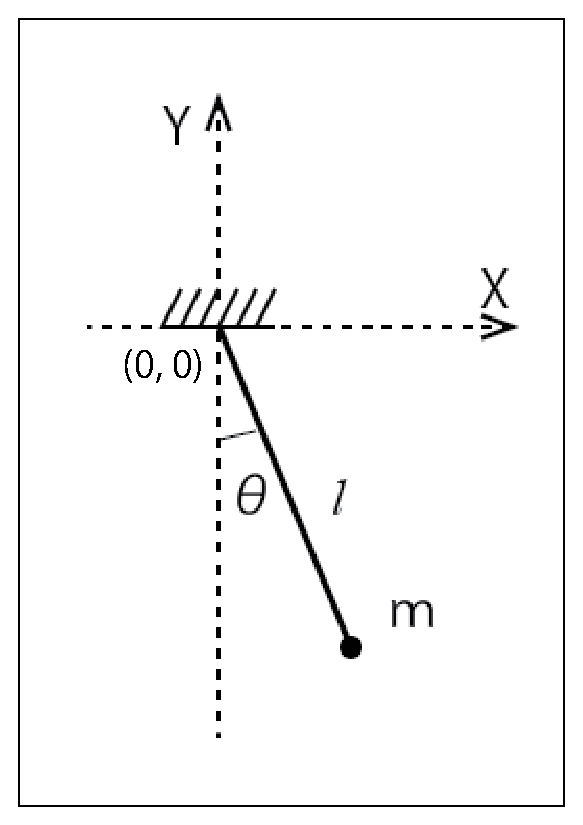
\includegraphics[keepaspectratio, scale=0.6]{eps/single.eps}
    \caption{単振子}
  \end{minipage}
  %\begin{minipage}[b]{0.45\linewidth}
    %\centering
    %\includegraphics[keepaspectratio, scale=0.35]{p13-2.eps}
    %\caption{p13-2}
  %\end{minipage}
\end{figure}
%\end{comment}

一方の端が固定され,質量を無視できる長さ$l$の棒の他端に,質量$m$の質点が拘束されている.棒が鉛直となす角は$\theta$,重力加速度は$g$である.

\[
\displaystyle T=\frac{1}{2}m(l\dot{\theta})^2,\quad U=-mgl\cos\theta
\]

より,Lagrangian$L=T-U$は,

\[
\displaystyle L=\frac{1}{2}ml^2\dot{\theta}^2+mgl\cos\theta
\]

Euler-Lagrange eq.は、

\[
\displaystyle\frac{\mathrm{d}}{dt}\frac{\partial L}{\partial \dot{\theta}}-\frac{\partial L}{\partial \theta}=0
\]

により次の通り.

\[
\displaystyle\ddot{\theta}=-\frac{g}{l}\sin\theta
\]

\section{Pythonで模擬実験}

これを次のように1階まで分解し,連立にして関数odeを定義する.\\

\begin{align*}
\displaystyle\frac{\mathrm{d}\theta}{\mathrm{d}t}&=\dot{\theta}\\\\
\displaystyle\frac{\mathrm{d}\dot{\theta}}{\mathrm{d}t}&=-\displaystyle\frac{g}{l}\sin\theta
\end{align*}\\

常微分方程式(Ordinary Differential Equation;ODE)の積分は,scipy.integrateのodeintを使う.関数odeの戻り値は,$[\theta,\dot{\theta}]$である.Pythonのアニメーションには,FuncAnimationを使う.

\lstset{escapechar=@,style=custompy}
\lstinputlisting[caption=単振子,label=pythonProgram1]{py/single.py}
